% !TEX root = atlas_latex.tex

%-------------------------------------------------------------------------------
% Body of the guide to the use of the ATLAS LaTeX package
%-------------------------------------------------------------------------------
\section{Introduction}
\label{sec:intro}
%-------------------------------------------------------------------------------

This collection of ATLAS \LaTeX\ templates, style files and documentation
can be used for papers, preprints and notes, both public and internal. 
All necessary files are collected in a single package called \texttt{atlaslatex}.
The package is available from the web pages of the Publication Committee~\cite{pubcom} and from 
Git~\cite{pubcom-git}.

The collection replaces and hopefully improves on the previous packages. 
In particular it supersedes:
\begin{itemize}\setlength{\parskip}{0pt}\setlength{\itemsep}{0pt}
\item \texttt{atlasnote-00-04-05}
\item \texttt{atlascover-00-00-11}
\item \texttt{atlaspreprint-00-00-05}
\item \texttt{atlasbib-00-00-04}
\end{itemize}
Section~\ref{sec:oldnote} summarises the changes that have been made and
how you can adapt your documents to use the new package.
Section~\ref{sec:oldcover} summarises the changes to the cover macros.

The package includes the \Package{atlasdoc} class, useful style files
and documentation of the package.
The package also defines a standard ATLAS style for papers.
This style should be used for paper drafts and for submission to the arXiv and the journal.
This option is the default. Add the option \Option{atlasstyle=false} to the \Package{atlasdoc} class if you do not want to use this style.
The documentation is provided as both PDF files and \LaTeX\ documents
that should provide examples of how to use the package and how to write
good \LaTeX.

The design principle is that you have a main document and 
the style files and \Package{atlasdoc} class are in a subdirectory \File{latex}.
The logos that are needed are kept in a \File{logos} directory.
This subdirectories can of course be links to a centrally maintained \texttt{latex} directory.
See below and Section~\ref{sec:texmf} for how to proceed if you want to use and/or install
the package in a central place.

The usual procedure is that for each document that you create,
you first unpack the latest version of \Package{atlaslatex} and
then create your main document in the top-level directory.
This structure means that it is easier to update the style files if a new version of
\Package{atlaslatex} is released. 
Each document can then be independent of the \Package{atlaslatex} release.

To create a new document you can issue the commands:
%
\begin{verbatim}
make new [BASENAME=mydocument] [TEXLIVE=YYYY]
\end{verbatim}
%
This command copies \File{atlas-document.tex} and
\File{atlas-document-metadata.tex}
to \File{mydocument.tex} and \File{mydocument-metadata.tex}.%
\footnote{The \File{Makefile} should work for regular Linux and MacOSX distributions.
  For Windows, you probably have to execute the tasks in the \File{Makefile} by hand.}
The selected \TeX\ Live version is set with the \Option{TEXLIVE} option. The default is 2016.
The \texttt{make} command also creates empty files \File{mydocument-defs.sty} and \File{mydocument.bib}.
By default the document will be an ATLAS note.
If you want it to be a paper draft, add the option \Option{PAPER} to the document class.
In the \File{Makefile} you should change the \texttt{BASENAME} to the name of your document.
You can then compile your document with the command: \texttt{make}.
Have a look at \File{Makefile} for other things you can adjust.

If you install \Package{atlaslatex} in a central directory such as \File{\$\{HOME\}/texmf} the basic command is:
%
\begin{verbatim}
make newtexmf [BASENAME=mydocument] [TEXLIVE=YYYY]
\end{verbatim}
%
See Section~\ref{sec:texmf} for more details.

In order to make a new document of book form like a TDR, use the command
%
\begin{verbatim}
make newbook [BASENAME=mydocument] [TEXLIVE=YYYY]
\end{verbatim}
%
By default, this will pass the option \Option{BOOK} to \Package{atlasdoc}.
Use \verb|make newbooktexmf| for a book with \Package{atlaslatex} in a central directory.

Note that you have to specify the language of your document as an option in the
\Macro{documentclass} command. Typical settings are
\begin{itemize}
\item UKenglish (or british);
\item USenglish (or american).
\end{itemize}

As mentioned above the default \TeX\ Live version is currently set to 2016.
This should be the only option you have to adjust if you use different versions of \LaTeX.
You can always set a version lower than the one you have installed to maintain compatibility with older versions.
To test compatibility with arXiv, try a setting of 2016.
%This will, among other things, automatically switch from the \Package{newtx} fonts to \Package{txfonts} if you
%are using the ATLAS preprint style.

As of Version 01-07-00 of \Package{atlaslatex} you should include the command \Macro{maketitle} after your\\
\verb|\begin{document}| if you want the document title to be printed.

Add the option \Option{atlasstyle=false} to the \Macro{documentclass} if you do not want to typeset your document in the ATLAS preprint style.


%-------------------------------------------------------------------------------
\section{Title, author and document numbers}
\label{sec:metadata}
%-------------------------------------------------------------------------------

An ATLAS document usually collects a series of labels over time.
These include the reference code of the analysis, e.g.\ \texttt{BPHY-2013-04}, 
the ATLAS note number and the CERN preprint number.
In addition the abstract and title are needed on the front page of the document and also on various cover pages.
The editors of the document, the editorial board members and the contributors to the analysis
also need to be specified at some point.

While all this information can be collected in the main file of the document, 
it is probably better to put it all in a separate document.
By default this file is called \texttt{mydocument-metadata.tex}.


%-------------------------------------------------------------------------------
\subsection{Authors and Contributors}
\label{sec:contribute}
%-------------------------------------------------------------------------------

The supporting documentation for an ATLAS note (not the paper draft) should contain a list of the contributors to the analysis.
A style file \Package{atlascontribute.sty} has been written to help with the creation of such a list.
The macros in the style file can also build the author list at the same time.
Two basic macros are used to add names to the author list and list of contributions:
\Macro{AtlasContributor} and \Macro{AtlasAuthorContributor}. 
The first macro adds a person to the list of contributors, while the second one also adds the person
to the author list. I assume that in almost all cases you will want to use \Macro{AtlasAuthorContributor}.
Typical commands are:
\begin{verbatim}
\AtlasAuthorContributor{Joe Student}{a}{fake background estimate.}
\AtlasAuthorContributor{Jane Student}{b}{top background estimate.}
\AtlasAuthorContributor{John Postdoc}{a}{editor of internal note.}
\AtlasContributor{Jo Helper}{useful contributions in a few places.}
\affil[a]{University of Nowhere}
\affil[b]{University of Somewhere}
\end{verbatim}
If a person should be added to the author list, you also need to add an appropriate affiliation using the macro \Macro{affil}.
The optional argument is a letter or number that should also be given as the second argument to
\Macro{AtlasAuthorContributor}.

You can keep the list of authors and contributors separate
by using \Macro{author} for the authors and \Macro{AtlasContributor} for the contributors.
You print the list of contributors by giving the command \Macro{PrintAtlasContribute}.
Note that \Macro{PrintAtlasContribute} has an argument that gives the fraction of the line width
to be used for the name of the person.
The list should either be printed before the table of contents or after the conclusions
(i.e.\ where the Acknowledgements appear in a paper).

Note that \Package{authblk} assumes that you will also have affiliations for each author.
You can avoid them by using the syntax \verb|\author{[ ]{Author Name}}|.
Note that a space is needed in the optional argument.
This means that a space appears between the author name and the comma after it, which is not so nice.
Alternatively you can make the author list using the syntax:\\
\verb|\author{Joe Student \and Jane Student \and John Postdoc}| and avoid the use of the
\Package{authblk} package by giving the option \Option{authblk=false} to \Package{atlascontribute}.

Note that the \Package{atlascontribute} package requires that the packages 
\Package{array} and \Package{booktabs} be installed.
If the list of contributors is very long, it may spread over more than one page.
The \Package{tabular} environment does not like this.
Add the option \Option{xtab} to use \Package{xtab} instead.
This option of course also requires that the package \Package{xtab} is installed.


%-------------------------------------------------------------------------------
\subsection{Special author lists}
%-------------------------------------------------------------------------------

Sometimes a PUB note has a special author list.
Hence a link to this list should be added to the front page.
This can be achieved with the following code snippet that should be used for the author:
\begin{verbatim}
% \usepackage[marginal,hang]{footmisc}
% \setlength{\footnotemargin}{0.5em}
\usepackage{authblk}
\author{The ATLAS Collaboration%
\thanks{The full author list can be found at:\\
  \url{https://atlas.web.cern.ch/Atlas/PUBNOTES/ATL-PHYS-PUB-2014-YYY/authorlist.pdf}}
}
\end{verbatim}

The first two lines are needed if you do not use the standard ATLAS preprint style.
Note that \Package{atlasdoc} has to be loaded with the option \Option{maketitle=false}
and \Macro{maketitle} should be added after \verb|\begin{document}|.
This is the default as of Version 01-07-00 of \Package{atlaslatex}.


%-------------------------------------------------------------------------------
\subsection{Metadata commands}
%-------------------------------------------------------------------------------

The standard list of metadata commands are given below.
More are available for the draft cover page when a paper, CONF note or PUB note draft
is circulated to the collaboration.\\
See \texttt{template/atlas-document-metadata.tex} for more details.

\begin{itemize}
  \item {\verb|\AtlasTitle{<Title>}|} typesets the paper title. If not
    given, you get either an error or a dummy title will be produced.

  \item {\verb|\author{<Author>}|} typesets the paper author. If not
    explicitly given, \enquote{The ATLAS Collaboration} will be used by
    default. Note that the \verb|\author{}| command is pretty limited
    in case you want to display multiple author names and multiple
    affiliations. For this use case the \verb|authblk.sty| package is
    provided; this is a typical example of its use:
    \begin{verbatim}
\usepackage{authblk}
\renewcommand\Authands{, } % avoid ``. and'' for last author
\renewcommand\Affilfont{\itshape\small} % affiliation formatting

\author[a]{First Author}
\author[a]{Second Author}
\author[b]{Third Author}

\affil[a]{One Institution}
\affil[b]{Another Institution}
    \end{verbatim}
    See also Section~\ref{sec:contribute} if you want to combine the creation of a list of authors and contributors.

  \item {\verb|\AtlasAbstract{<The abstract text>}|} typesets the
    abstract on the front page and cover page.

  \item {\verb|\date{<Date>}|} typesets the paper date. If not
    explicitly given, the current date (\verb|\today|) will be used.

  \item {\verb|\AtlasVersion{<Draft Version>}|} displays the draft
    version on the front page, a DRAFT banner on all the other page
    headings, and adds line numbers to all text to easy commenting and
    reviewing.
    Should be included when paper draft is circulated to ATLAS.
    Highly recommended for all documents in the draft stage.

  \item {\verb|\AtlasJournal{<Journal Name>}|} displays the phrase \emph{to
    be submitted to Journal Name} at the bottom of the front page and
    on the cover page.
    Should be included when a paper draft is circulated to ATLAS.

  \item {\verb|\AtlasRefCode{<Reference code>}|} displays the ATLAS
    standard reference code, e.g.\ \texttt{BPHY-2014-03}, on the front page and
    the cover page. Not shown on the front page if the note number is given.

  \item {\verb|\AtlasNote{<Note number>}|} displays the note number
    for a CONF, PUB, INT or COM note, e.g.\ \texttt{ATLAS-CONF-2014-23},
    on the front page and cover page.
    If the note number is given, the reference code is not shown.

  \item {\verb|\PreprintIdNumber{<CERN preprint number>}|} displays the CERN
    preprint number on the front page.
    
  \item {\verb|\AtlasDate{<Date>}|} set by the Physics Office as the date of submission of a paper.

  \item {\verb|\AtlasJournalRef{<Journal reference>}|} displays the journal reference
    on the preprint front page.
    This should be used for the arXiv update after the paper has been published.

  \item {\verb|\AtlasDOI{<Journal reference>}|} displays the DOI
    on the preprint front page.
    This should be used for the arXiv update after the paper has been published.

  \item {\verb|\arXivId{<arXiv identifier>}|} displays the arXiv reference
    on the front page.

\end{itemize}
%
\texttt{template/atlas-document.tex} contains a basic skeleton that can be
used to start typing a new note using the \texttt{atlasdoc} class. Many of
the custom commands described above are used in this example file, in
order to demonstrate their use.

Links to supporting documentation should also be included on the cover page of draft papers circulated to ATLAS.
They can be included using
\verb|\AtlasCoverSupportingNote{Short title}{CDS link}|.
It is also possible to give a TWiki page instead, but this is deprecated.\\
As mentioned above, see \texttt{template/atlas-document-metadata.tex} for more details.


%-------------------------------------------------------------------------------
\section{The \texttt{atlasdoc} class}
\label{app:atlasdoc}
%-------------------------------------------------------------------------------

This document has been typeset using the \texttt{atlasdoc.cls} class.

The \texttt{atlasdoc} class can use either the standard \LaTeX\ \texttt{article} class
as its basis or the \KOMAScript\ \texttt{sctartcl} class.
All the usual commands and options you usually use
with \texttt{article}  or \texttt{scrartcl} should work with it. 
You turn on the use of \KOMAScript\ with the option \texttt{koma}.
For instance, this document has
been produced using this very simple preamble:
%
\begin{verbatim}
  \documentclass[UKenglish]{latex/atlasdoc}
  \usepackage{latex/atlaspackage}
  \usepackage{latex/atlasphysics}
  \graphicspath{{../../logos/}{figures/}}
\end{verbatim}
%
Note that the document language must be specified, otherwise \texttt{babel} will complain.

The \LaTeX\ packages that are used in the document are mostly specified in 
\texttt{latex/atlaspackage.sty}.

The style file \texttt{latex/atlasphysics.sty} defines a lot of useful
macros for particles and more. See the separate document
\texttt{atlas\_physics.pdf}~\cite{atlas-physics} for details.

If you do not want to use \Package{biblatex} you need to add the option \Option{biblatex=false} when you
include \texttt{atlaspackage}.
Have a look at the \texttt{latex/atlaspackage.sty} to see how \texttt{biblatex} is included.
In your main document you use \Macro{addbibresource} in the preamble to include your \texttt{.bib} files.
Note that the backend \Package{biber} returns with an error if it finds an empty \texttt{.bib} file.
A style file \File{latex/atlasbiblatex.sty} is available that adjusts the format of the references to the usual ATLAS conventions.

As mentioned above, you have to specify the document language as an option to \Package{atlasdoc}.
Several more options can be set.
In the following the default option is in boldface.
\begin{description}
\item[\Option{atlasstyle=true|{\normalfont false}}] turn on (default) or off the use of the ATLAS style for the document;
\item[\Option{coverpage}] include an ATLAS draft cover page;
\item[\Option{cernpreprint}] make the front page for a CERN preprint.
  The option \Option{preprint} works as well, but is deprecated;
\item[\Option{NOTE}] the document is an ATLAS note (default);
\item[\Option{PAPER}] the document is an ATLAS paper (draft);
\item[\Option{CONF}] the document is a CONF note;
\item[\Option{PUB}] the document is an PUB note;
\item[\Option{BOOK}] the document is book form like an LOI or TDR;
\item[\Option{auxmat}] the document contains auxiliary material for a preprint;
\item[\Option{texlive=2016}] adjust if you use an older version of \TeX\ Live like 2011.
  A value less than 2013 adjusts a few \Package{biblatex} options.
  A value less than 2012 uses \Package{txfonts}.
\item[\Option{paper=a4|{\normalfont letter}}] set the paper size;
\item[\Option{titlesize=normal|{\normalfont small}}] use normal or reduced size fonts for the title page;
\item[\Option{floatopt=true|{\normalfont false}}] adjust the options (default) governing number and placement of floats on a page;
\item[\Option{texmf}] use the syntax \Macro{usepackage\{package\}}
  instead of \Macro{usepackage\{latex/package\}} to include packages.
  This is needed if you install \Package{atlaslatex} centrally,
  rather than in a \File{latex} subdirectory;
\item[\Option{newtx}] use the \Package{newtxtext} and \Package{newtxmath} packages for fonts 
  (default for \TeX Live > 2012);
\item[\Option{txfonts}] use the \Package{txfonts} package for fonts instead of the default
  (default for older \TeX Live versions);
\item[\Option{mhchem={\normalfont true}|false}] include \Package{mhchem} before \Package{xpatch} to avoid
  an error with \TeX\ Live 2014;
\item[\Option{datetop=true|{\normalfont false}}] use normal or smaller fonts on the title page;
\item[\Option{showframe={\normalfont true}|false}] load the \Package{showframe} package, to display frames showing the boxes for text body, header, footer and margin;
\item[\Option{titleextraheight=0em}] extra height that could be needed for the title, if it is very long;
\item[\Option{copyrightoffset=0em}] adjust the position of the copyright,
  if it is not completely correct.
\end{description}

The following options were removed in \Package{atlasdoc} in \Package{atlaslatex 02-00-00}.
They are mostly still available in \Package{atlasdoc1}.
\begin{description}
\item[maketitle={\normalfont true}|false] turn on or off the creation of a title page within \Macro{AtBeginDocument}.
  If the option is false, but you still want a title, give the command \Macro{maketitle} after
  \verb|\begin{document}|.
  This is the recommended way of proceeding;
\item[nomaketitle] do not create a title page; equivalent to \Option{maketitle=false}.
  This option has no effect as of \Package{atlaslatex} 01-07-00 of \Package{atlaslatex};
\item[koma=true|{\normalfont false}] use the \KOMAScript\ base class \Package{scrartcl} instead of \Package{article};
\item[\Option{letterpaper}] set the paper size to letter.
\item[\Option{a4paper}] set the paper size to A4;
  \emph{This option was removed in \Package{atlaslatex} 02-00-00
  -- use \Option{paper=a4} instead};
\item[\Option{letter}] set the paper size to letter.
  \emph{This option was removed in \Package{atlaslatex} 02-00-00
  -- use \Option{paper=letter} instead};
\end{description}
Note that the options \Option{CONF} and \Option{PUB} get passed to \Package{atlascover.sty}
as they only influence the cover pages.
%The option \Option{BOOK} uses book intead of article as the base class.

The
\href{http://www.tex.ac.uk/cgi-bin/texfaq2html?label=floats}{UK List of FAQ}
recommends changing several default \LaTeX\ options so that there are fewer problems
with figure and table placement.
It is certainly worth reading that page for further advice.
As it is very hard to really test how well these options work
they can be turned on or off in \Package{atlasdoc} via the option \Option{floatopt=true|false}.
The default value is set to \Option{true}.

As of \Package{atlasdoc} Version 02-00-00,
the \KOMAScript elements are used to create the title pages.
In particular, \Macro{publishers} is used for the abtract and copyright.
The space and position for this may need to be adjusted,
if you have a very long title. Use the options
\Option{titleextraheight} and \Option{copyrightoffset} to make adjustments.
It is very helpful to turn on the \Option{showframe} option when doing this.


%-------------------------------------------------------------------------------
\subsection{Dependencies and \Package{atlaspackage}}
\label{sec:atlaspackage}
%-------------------------------------------------------------------------------

The \Package{atlasdoc} class depends on these packages, whose presence in
your system is required:
\begin{itemize}\setlength{\parskip}{0pt}\setlength{\itemsep}{0pt}
\item \Package{babel}: become language aware;
\item \Package{fancyhdr} or \Package{scrpage2}: defines the header for draft mode
  and for auxiliary material documents.
  \Package{fancyhdr} is used for the standard \LaTeX\ classes and
  \Package{scrpage2} for \KOMAScript;
\item \Package{fontenc}: output font encoding;
\item \Package{hyperref}: add hyperlinks and ability to click on cross-references;
\item \Package{graphicx}: include graphics in the document;
\item \Package{lineno}: add line numbers to documents;
\item \Package{newtxtext} and \Package{newtxmath}: the standard ATLAS document font.
  If this is not available, you can fall back to \Package{txfonts};
\item \Package{xcolor}: add colours to \LaTeX;
\item \Package{ifthen}: improved handling of conditionals.
%\item \Package{scrdate, scrtime}: Current date and time for use in the header.
\end{itemize}
These should be installed in any modern \LaTeX\ installation.
See \cite{latex-faq} for details on which collections are needed to get these packages
for your operating system.

Note that under Ubuntu versions 12.04 and 14.04, \Package{lineno} can be found in the
\Package{texlive-humanities} package!
If you cannot find it, it is also included in \File{latex/other}.
Copy it to your main directory, or to \verb|${HOME}/texmf/tex/latex| in order to make
it centrally available.

Both the class \Package{atlasdoc} and all style files:
\Package{atlasbiblatex}, \Package{atlascontribute}, \Package{atlascover}, \Package{atlaspackage} and \Package{atlasphysics},
need the package \Package{kvoptions} 
so that they can process options where a value for an option should be set.

\Package{atlasdoc} and \Package{atlascover} both need \texttt{hyperref}. 
Have a look at one of these packages to see how to include it by hand.
You can also simply use \texttt{atlaspackage.sty}

The style file \texttt{atlaspackage.sty} includes further packages.
You can steer how many by using the option \Option{minimal}, \Option{default} or \Option{full}.
The minimal set is:
\begin{itemize}\setlength{\parskip}{0pt}\setlength{\itemsep}{0pt}
\item \texttt{amsmath}: extra useful maths environments;
\item \texttt{inputenc}: allow ä, ö, ø, ß, etc. to be input directly;
\item \texttt{hyperref}: add hyperlinks and ability to click on cross-references;
\item \texttt{placeins}: adds commands to force figure and table output before a certain position in the text.
\end{itemize}

The default set adds in addition:
\begin{itemize}\setlength{\parskip}{0pt}\setlength{\itemsep}{0pt}
\item \texttt{booktabs}: nicer tables. Use \Macro{toprule}, \Macro{midrule} and \Macro{bottomrule} instead of \Macro{hline};
\item \texttt{csquotes}: smart quotes that incorporate language dependence;
\item \texttt{siunitx}: units package with extra functionality for tables;
\item \texttt{subfig}: more than one plot in a figure;
\item \texttt{tocloft}: extra options for typesetting table of contents etc.
\end{itemize}

Finally the full set includes further packages that may be useful:
\begin{itemize}\setlength{\parskip}{0pt}\setlength{\itemsep}{0pt}
\item \texttt{mhchem}: chemical elements and molecules;
\item \texttt{rotating} rotate figures, tables, etc.;
\item \texttt{xfrac} nicer fractions;
\item \texttt{xtab} newer version of \Package{supertabular}, which allows tabular environments to go over more than one page.
\end{itemize}

The full list of options is:
\begin{description}\setlength{\parskip}{0pt}\setlength{\itemsep}{0pt}
\item[\Option{biblatex=true|{\normalfont false}}] turn on/off use of \Package{biblatex} and \Package{biber/bibtex};
\item[\Option{backend=bibtex|{\normalfont biber}}] specify the backend to use with \Package{biblatex}.
  Specify \Option{backend=biber} to use \Package{biber} instead;
\item[\Option{hyperref=true|{\normalfont false}}] turn on/off use of \Package{hyperref};
\item[\Option{siunitx=true|{\normalfont false}}] do not include the \Package{siunitx} package;
\item[\Option{eVkern={\normalfont true}|false}] apply a kern of -0.1em to \si{\eV} in order to move \enquote{e} and \enquote{V} closer together.
  This option is set by default if you use the \Option{txfonts} fonts;
\item[\Option{csquotes=true|{\normalfont false}}] do not include the \Package{csquotes} package;
\item[\Option{subcaption={\normalfont true}|false}] use \Package{subcaption} instead of \Package{subfig};
  \Package{subcaption} is supposed to be a newer, better and more general package than \Package{subfig} or
  \Package{subfigure}.
  It is probably best to only use it with \TeX\ Live 2012 or later;
\item[\Option{subfigure={\normalfont true}|false}] use the deprecated package \Package{subfigure} 
  instead of \Package{subfig};
\item[\Option{subfig=true|{\normalfont false}}] use the somewhat deprecated package \Package{subfig};
\item[\Option{texlive=2016}] set if you use an older version of \TeX\ Live like 2011.
  A value less than 2013 adjusts a few \Package{biblatex} options.
  A value less than 2012 uses \Package{txfonts} and the old (Version 1) option names for \Package{siunitx}.
  A value less than 2010 uses the old option names for \Package{csquotes}.
  Use \Option{texlive=2016} to test options for arXiv submissions;
\item[\Option{txfonts={\normalfont true}|false}] load the \Package{txfonts} package and adjust loading of \Package{amsmath} for duplicate symbols;
\item[\Option{lineno={\normalfont true}|false}] load the \Package{lineno} package.
\end{description}

\File{lineno.sty} and \File{authblk.sty} are also provided in \File{latex/other}.
They should be part of a standard \LaTeX\ installation though.

Depending on the font you use, you may find that the \enquote{e} and \enquote{V} in \si{\eV}, \si{\MeV} etc.\
are too far apart.
You can pass the option \Option{eVkern} to \Package{atlaspackage} in order to move them 0.1em closer together.\footnote{%
This option has no effect for \TeX\ Live 2011 and older, as \Package{siunitx}
adjusted the spacing internally using the parameter \Option{eVcorra}.}
This is the amount used in the \File{atlasunit.sty} for \Macro{gev} etc.
which is included by passing the option \Option{unit=true} to \Package{atlasphysics}.
If you use \Package{siunitx}, I recommend setting \Option{unit=false},
so that you use one consistent set of definitions throughout your document.

There used to be a problem using the \Package{tikz} package with \Package{atlasnote}.
With \Package{atlasdoc} this problem seems to have gone away.
\Package{tikz} is not included in \Package{atlaspackage}.
If you want to use it, just add the usual \verb|\usepackage{tikz}| to your preamble.

Other packages that have been used at some point include:
\begin{description}\setlength{\parskip}{0pt}\setlength{\itemsep}{0pt}
\item \Package{savesym}: needed to avoid errors if \Package{txfonts} is used, 
  as \Package{txfonts} and \Package{amsmath} define the same symbols;
\item \texttt{footmisc}: extra footnote options. 
  These mess up the \Option{atlasstyle} settings.
\end{description}


%-------------------------------------------------------------------------------
\subsection{Cover pages}
\label{sec:cover}
%-------------------------------------------------------------------------------

The package also provides cover pages for the circulations of ATLAS drafts and 
for the front page for the CERN preprint version of an ATLAS paper.
A further cover page is provided for a document containing auxiliary material associated with a preprint/paper.
The style file can be found in \texttt{latex/atlascover.sty}.

If you wish to use the \texttt{atlascover} package with the 
\texttt{atlasdoc} class, you should usually use the \texttt{coverpage} option of the class:
\begin{verbatim}
  \documentclass[coverpage,UKenglish]{latex/atlasdoc}
\end{verbatim}
instead of the the usual \texttt{usepackage} command: this will ensure
that the cover page is produced before the title page of the document.

You can include \texttt{atlascover} with \Macro{usepackage} if you prefer.
In this case you need the option \texttt{maketitle=false}
(which is the default as of Version 01-07-00 of \Package{atlaslatex}) in the \texttt{atlasdoc} class
(if you are using it)
and you include the \Macro{maketitle} command after \verb|\begin{document}|.

The following options can be passed on to the \Package{atlascover} package:
\begin{description}
\item[\Option{coverpage}] outputs the standard ATLAS paper draft cover page;
\item[\Option{CONF}] the document is a CONF note;
\item[\Option{PUB}] the document is an PUB note;
\item[\Option{cernpreprint}] the title page should be in the form of a CERN preprint;
  The option \Option{preprint} works as well, but is deprecated;
%\item[\Option{preprint}] the title page should be in the form of a CERN preprint;
\item[\Option{auxmat}] the title page for a document containing auxiliary material from a paper;
\item[\Option{coverfontsize}] the base font size used for the cover (default is 11pt). Adjust this for long abstracts;
\item[\Option{twocolumn}] use this option if your document is formatted in two columns;
\item[\Option{atlasdoc}] this option is set by \Package{atlasdoc} and is not usually needed by the user.
\end{description}

If you use \Package{atlascover} standalone, use the option \Option{coverpage=true} to
actually output a cover page. 
This is necessary as of Version 01-04-00 of \Package{atlaslatex} to make the use of options more consistent.
As of Version 02-00-00, the options \Option{cernpreprint}, \Option{preprint} and \Option{auxmat} are no longer available
in \Package{atlascover}.
You should pass these to \Package{atlasdoc} instead, as the title pages are now part of the main class.

Some papers have a very long abstract, such that it does not fit on the cover page.
You can reduce the font size used on the cover by setting the option \Option{coverfontsize}.
The default value is 11pt. Try 10.5pt or 10pt instead to get the abstract onto the page.

It used to be the case that some journal styles, especially JHEP,
produced an ATLAS draft cover page that was offset.
You could use the options \Option{hoffset} and \Option{voffset} to move the text around.\\
JHEP needed \verb|hoffset=1in, voffset=1in|.\\
revtex (APS journals) looked better with  \verb|hoffset=-0.25in, voffset=-0.25in|.\\
These offsets are ignored, as of Version 01-04-00 of \Package{atlaslatex},
as the problems with spurious offsets have been eliminated.

The option \Option{clearpage}, which used to exist, has no effect.


%-------------------------------------------------------------------------------
\section{The ATLAS preprint style}
\label{sec:atlasstyle}
%-------------------------------------------------------------------------------

This style should be used for the preparation of paper drafts,
as well as for the submission of papers to the arXiv and journals.
The journals will then convert the documents to the style appropriate for the journal.
As some experience has to be gained with this package,
feedback on any problems that occur with the style are very welcome.

Documents are typeset by default in the standard ATLAS preprint style.
The use of this style can be turned off by using the option
\Option{atlasstyle=false}.
This style uses \KOMAScript\ as the base class.
Further settings include:
\begin{description}
\item[Layout:] \Option{DIV=14} and an extra \SI{5}{\mm} for the binding;
\item[Paragraph:] The paragraph indentation is set to zero and 
  there is a half-line separation between paragraphs.
\item[Figures and tables:] a small font size is used for the captions.
  Captions are not indented.
  They should be below both figures and tables;
\item[Font:] the default fonts are from the \Package{newtx} package.
  These are very similar to \Package{txfonts} that have been used up to now,
  but have a better spacing in a few cases;
\item[Section headers:] the standard serif font is used.
\end{description}

The default fonts for ATLAS documents are \Package{newtxtext} and \Package{newtxmath}.
These are more modern variants of the package \Package{txfonts} that has been used in
ATLAS documents in the past.
%However, arXiv currently uses an older version of \TeX\ Live (2011) that does not include the
%\Package{newtx} fonts. 
%In ATLAS papers, please add the option \Option{texlive=2011} to \Package{atlasdoc}.
%As soon as arXiv switches to a newer version of \TeX\ Live this option may have to be adjusted
%or will no longer be necessary.

In general, if you have problems with the \Package{newtx} fonts,
you can switch to \Package{txfonts} by including the option \Option{txfonts} with \Package{atlasdoc}.


%-------------------------------------------------------------------------------
\section{CERN preprint and arXiv}
\label{sec:preprint}
%-------------------------------------------------------------------------------

If you are writing an ATLAS paper and it has been approved by the collaboration,
you have to make a version with the CERN preprint title page before submitting the paper to arXiv.
You do this by replacing the option \Option{PAPER} by \Option{cernpreprint} in \Package{atlasdoc}.
The CERN preprint number is given via the macro \Macro{PreprintIdNumber}.
At the same time you should pass the option \Option{texlive=2016} to
\Package{atlasdoc}.
This is because arXiv contains a 2016 \TeX\ Live installation.
Summarising, a typical \Macro{documentclass} command would be:
\begin{verbatim}
\documentclass[cernpreprint,texlive=2016,UKenglish]{latex/atlasdoc}
\pdfoutput=1
\end{verbatim}
The \Macro{pdfoutput} command tells arXiv that a PDF file should be produced directly.
You should also turn off ATLAS draft cover page -- remove the option \Option{coverpage=true}.
If you move the class and style files to the same directory as the main file,
you need to add the option \Option{texmf} to the \Macro{documentclass}.

You can test whether your document compiles with \TeX\ Live 2016 by setting your \texttt{PATH} on \texttt{lxplus} to
\begin{verbatim}
export PATH=/afs/cern.ch/sw/XML/texlive/2016/bin/x86_64-linux:$PATH
\end{verbatim}

Note that you should submit the \File{bbl} file and not the \File{bib} to arXiv.
Depending on which journal you submit to, you should turn on or off the printing of the titles in the bibliography.
Further details on how to proceed can be found on the Physics Office TWiki~\cite{atlas-physicsoffice} -- see
the Section on \enquote{Guidelines for paper submission}.
APS journals have special requirements on the directory structure and the filenames for figures.
%JINST uses a very old version of \LaTeX\ (2004).
Neither \Package{biblatex} nor \Package{siunitx} are available
and \KOMAScript\ does not contain the \Macro{KOMAoptions} command.
See the Physics Office TWiki~\cite{atlas-physicsoffice} for more information.

It also makes sense to clean up the metadata file at this point.
You get rid of line numbering by making sure that neither \Macro{AtlasVersion} nor \Macro{draftversion} are defined.
I recommend moving the relevant definitions into the main \TeX\ file so that the metadata file is no longer needed.
If you clean things up, the \Package{atlascover} package is no longer needed.
The metadata commands that are needed in addition to the title, author and abstract are:
\begin{itemize}
  \item {\verb|\AtlasJournal{<Journal Name>}|}
  \item {\verb|\PreprintIdNumber{<CERN preprint number>}|}
  \item {\verb|\AtlasDate{<Date>}|} set by the Physics Office
  \item {\verb|\AtlasJournalRef{<Journal reference>}|} once it exists
  \item {\verb|\AtlasDOI{<Journal reference>}|} once it exists
  \item {\verb|\arXivId{<arXiv identifier>}|} once it exists
\end{itemize}

More details on arXiv recommendations can be found at
\url{https://arxiv.org/help/submit_tex}.


%-------------------------------------------------------------------------------
\section{ATLAS notes}
\label{sec:note}
%-------------------------------------------------------------------------------

If you include the macro \Macro{AtlasNote} in your preamble,
the note number will be printed under \enquote{ATLAS NOTE} at the top of your document.
This can be used for any sort of ATLAS note, including CONF, PUB and INT notes.


%-------------------------------------------------------------------------------
\section{Auxiliary material}
\label{sec:auxmat}
%-------------------------------------------------------------------------------

Some papers have many pages of extra tables and plots that are mainly of use to theorists
who need extra information.
Such material can be collected in a separate document.
The front page for this document is formatted using the \Option{auxmat} option.
If you use this option you should specify the arXiv preprint identifier
using the macro \Macro{arXivId} and the HepData record using the macro
\Macro{HepDataRecord}.
This information is then included on the cover page in the form of clickable links.

Use of this option also adds the arXiv preprint identifier to the top of every page
of the document.

If you want to create an auxiliary material document with an older \TeX\ Live version such as 2009, 
use the command \texttt{make auxmat TEXLIVE=2009}.


%-------------------------------------------------------------------------------
\section{Symbols in \texttt{atlasphysics.sty}}
\label{sec:atlasphysics}
%-------------------------------------------------------------------------------

Many useful symbols are defined in \texttt{atlasphysics.sty}.
While this used to be a very long file, it has now been split into several smaller files,
which can be included or not using options.
The definitions can be found in a separate document \File{atlas\_physics.pdf}.


%-------------------------------------------------------------------------------
\section{\texttt{atlaslatex} directories and Git or SVN}
\label{sec:gitsvn}
%-------------------------------------------------------------------------------

There is some flexibility in how you set up your directory structure for using \Package{atlaslatex}.
By default the \Package{atlaslatex} style files are in the \File{latex} subdirectory and the
logos are in \File{logos}. This structure assumes that you will make a separate directory tree
for each document that you create. If you want to include these files in Git or SVN, note that you only need to add the
\File{latex}, \File{logos} and \File{bibtex} directories of the \Package{atlaslatex} package to Git or SVN.

If you want use a centrally installed \texttt{atlaslatex} package, then you would usually unpack the\\
\File{atlaslatex-XX-YY-ZZ.tds.zip} file into your \File{texmf} tree -- see Section~\ref{sec:texmf}.

If you want to use another setup, you should set the variable \Macro{ATLASLATEXPATH} appropriately
at the beginning of your document. This would enable you to maintain a single copy of each 
\Package{atlaslatex} version and easily switch between versions.
For example, you give the command\\
\verb|\newcommand*{\ATLASLATEXPATH}{../atlaslatex-01-08-00/}|
to use version 01-08-00 of the \Package{atlaslatex} package, which you have unpacked into the directory tree
\File{../atlaslatex-01-08-00}.
Such a structure makes it very easy to switch between \Package{atlaslatex} versions without breaking anything!


%-------------------------------------------------------------------------------
\section{Installation of \Package{atlaslatex} in \File{texmf} tree}
%-------------------------------------------------------------------------------
\label{sec:texmf}

As discussed above, the \texttt{atlasdoc} class and the style files can all be found in the 
\File{latex} subdirectory. The template documents are usually set up to pick up the style files from there.
If you want to use the centrally installed version,
you should first copy \File{Makefile} and the \File{template} directory from 
\File{\$\{HOME\}/texmf/source/atlaslatex} to the directory where you want to create your document.
For the main document, you can then use the command \texttt{make newtexmf} to get a template which uses the
centrally installed style files.

If you want to install the package in a central area, use the \File{atlaslatex-XX-YY-ZZ.tds.zip} file.
Change your directory to \File{\$\{HOME\}/texmf} and unzip the file there. To do it by hand you can do:
\begin{itemize}
\item unpack the tarball;
\item copy the \texttt{latex} directory to \File{\$\{HOME\}/texmf/tex/latex/atlaslatex};
\item copy the contents of the \File{bibtex/bst} and \File{bibtex/bib} directories 
  to \texttt{\$\{HOME\}/texmf/bibtex/bst} and \texttt{\$\{HOME\}/texmf/bibtex/bib}, respectively.
\end{itemize}
It is more complicated to checkout part of a Git repository.
Hence the method described above is the recommended way of installing
\Package{atlaslatex} in your \File{texmf} tree.
% You can also checkout the two directory trees from SVN:
% {\small
% \begin{verbatim}
% cd ~/texmf/tex/latex
% svn co svn+ssh://svn.cern.ch/reps/atlasgroups/pubcom/latex/atlaslatex/trunk/latex atlaslatex
% cd ~/texmf
% svn co svn+ssh://svn.cern.ch/reps/atlasgroups/pubcom/latex/atlaslatex/trunk/bibtex
% \end{verbatim}
% }
% The advantage of using SVN is that you can keep the package up to date, by just giving the command
% \verb|svn update| in the two directories.
% If you already have a \File{bibtex} directory,
% first move it out of the way, then checkout from SVN
% and then move the contents of the old directory back into the \File{bibtex} tree.

% Under Windows, it appears to be better to use \texttt{https} instead of \texttt{svn+ssh}.
% You should therefore checkout:\\
% \verb|https://svn.cern.ch/reps/atlasgroups/pubcom/latex/atlaslatex/trunk|

In the template files, you have to use the command \texttt{make newtexmf} or change
\begin{center}
  \begin{tabular}{ll}
    From & To \\
    \midrule
    \verb|\documentclass{latex/atlasdoc}|    & \verb|\documentclass[texmf]{atlasdoc}| \\
    \verb|\usepackage{latex/atlaspackage}|   & \verb|\usepackage{atlaspackage}| \\
    \verb|\usepackage{latex/atlasbiblatex}|   & \verb|\usepackage{atlasbiblatex}| \\
    \verb|\usepackage{latex/atlascontribute}| & \verb|\usepackage{atlascontribute}| \\
    \verb|\usepackage{latex/atlasphysics}|   & \verb|\usepackage[texmf]{atlasphysics}|
  \end{tabular}
\end{center}

If you are using traditional \BibTeX\ you also have to change\\
\verb|\bibliographystyle{bibtex/bst/atlasBibStyleWoTitle}| to\\
\verb|\bibliographystyle{atlasBibStyleWoTitle}|

The \Option{texmf} option in \Package{atlasphysics} is not strictly necessary if you use the class \Package{atlasdoc},
but it does not do any harm.


%-------------------------------------------------------------------------------
\section{Platforms and \LaTeX\ versions}
\label{sec:version}
%-------------------------------------------------------------------------------

The \Package{atlasdoc} class works both with \LaTeX{} and pdf\LaTeX{}.
I recommend to use pdf\LaTeX\ and this is the default.

I would expect everything to work with \TeX\ Live 2009 or later.
You should just set the option \Option{texlive} appropriately.
This is best done in the document class, as the option is then passed to all other packages.
Examples of changes include some option names for \Package{siunitx},
and \Package{biblatex} and \Package{biber} were not really stable in earlier years.

If for example you have \TeX\ Live 2009, add the option \Option{texlive=2009} to the document class.
This will then include \Package{siunitx} with the correct options for Version 1.
It will also switch to \Option{unit=false} to \Package{atlasphysics}
and use option \Option{txfonts} in \Package{atlasdoc}.
If you want to use \Package{biblatex},
the current default for all years is to use the \Package{bibtex} backend rather than \Package{biber}.
You can use \Package{biber} instead by passing the option \Option{backend=biber} to \Package{atlaspackage}.

The \Package{atlaslatex} package should work under Linux, MacOSX and Windows.
Details on the installations that I use for testing things
and how you should set up your system can be found on the PubCom LaTEX FAQ~\cite{latex-faq}.


%-------------------------------------------------------------------------------
\section{Miscellaneous \LaTeX{} tips}
%-------------------------------------------------------------------------------
\label{sec:latex}

%-------------------------------------------------------------------------------
\subsection{Line numbers}

Line numbers can be printed using the \Package{lineno} package, 
which is included by default.
Line numbers are automatically turned on if you set \Macro{AtlasVersion} (or \Macro{draftversion}).
In general, you can turn them on and off in a document by using the \Macro{linenumbers} or \Macro{nolinenumbers} commands.
Note that if \Macro{AtlasVersion} is set, you will always get line numbers on the standard title page.
Hence, for CONF and PUB notes it is important to comment out \Macro{AtlasVersion} in order to suppress the line numbers for the final version.

In order to avoid line numbers going slightly wrong around figures and tables,
separate the \Package{figure} and \Package{table} environment from the rest of the text using blank lines.

If you use AMS Math \LaTeX\ environments such as \Package{align} line numbering may be interrupted around the environment.
Enclose the environment in a \Package{linenomath} environment to fix this problem:
\begin{verbatim}
\begin{linenomath}
\begin{equation*}
  E = m c^{2}
\end{equation*}
\end{linenomath}
\end{verbatim}


%-------------------------------------------------------------------------------
\subsection{Definitions}

You can use \verb|\ensuremath| in definitions, so that they will work
in both text mode and math mode, e.g.\
\verb|\newcommand{\UoneS}{\ensuremath{\Upsilon(\text{1S})}\xspace}| to get
\UoneS in either mode (\verb|\UoneS{}| or \verb|$\UoneS$|).

I highly recommend that you also terminate every definition with \Macro{xspace},
as then you can use the definitions without having to terminate them with
\enquote{\textbackslash\textvisiblespace} or \enquote{\{\}}.


%-------------------------------------------------------------------------------
\subsection{Figures}

Use the \Package{graphicx} package to include your plots and figures. 
The use of older packages like \Package{espfig} is deprecated.
Since the \Package{graphicx} package is required by the \Package{atlasdoc}
class, it is automatically loaded when using it, and there is no need
to explicitly include it in the document preamble.

Always include your graphics file without giving the file extension.
For instance, if you want to include the \File{figure.eps}
file, you should use a syntax like this:
\begin{verbatim}
  \includegraphics[width=\textwidth]{figure}
\end{verbatim}
This will allow you to compile your document using either \LaTeX{} or
pdf\LaTeX{} without changing your source file: you can in fact have
both \File{figure.eps} and \File{figure.pdf} in your working directory,
and the proper one will be picked up according to the processing method
you choose.

Figures should be in general be made available in both \texttt{eps} (or \texttt{pdf}) and 
\texttt{png} format. Additionally, a \texttt{pdf} version of the plots can be
useful in case \verb|pdflatex| is used to produce a publication.
%Colour versions are appropriate for talks, and black-and-white
%versions are necessary for the publication itself.

It is a good habit to keep your graphics files in a separate
sub-directory (e.g.\ in \File{figures/}. 
In this case you can include them by mentioning it explicitly every time:
\begin{verbatim}
  \includegraphics[width=\textwidth]{figures/figure}
\end{verbatim}
or by telling the \Package{graphicx} package where to look
for them, by using this command:
\begin{verbatim}
  \graphicspath{{figures/}}
\end{verbatim}

If you use a modern version of \TeX\ Live, it creates PDF files automatically from EPS files
(if they do not exist) when you use \File{pdflatex}.
An EPS file with the name \File{picture1.eps} will lead to a PDF file with the name
\File{picture1-eps-converted-to.pdf}.
If you have a lot of figures in many different directories, you may want to clean up the PDF files every so often.
You can use the command \verb|make cleanepstopdf| to achieve this.
You should adjust the top-level figures directory in the \File{Makefile} accordingly.


%-------------------------------------------------------------------------------
\subsection{Subfigures}

An example figure can be seen in Figure~\ref{fig:example}.
The standard options to use for the positioning are \Option{htbp}.
If you get a couple of lines of text at the top of the page,
make sure the figure is separated from the rest of the text with blank lines and/or try dropping the \Option{h} option.

\begin{figure}[htbp]
  \centering
  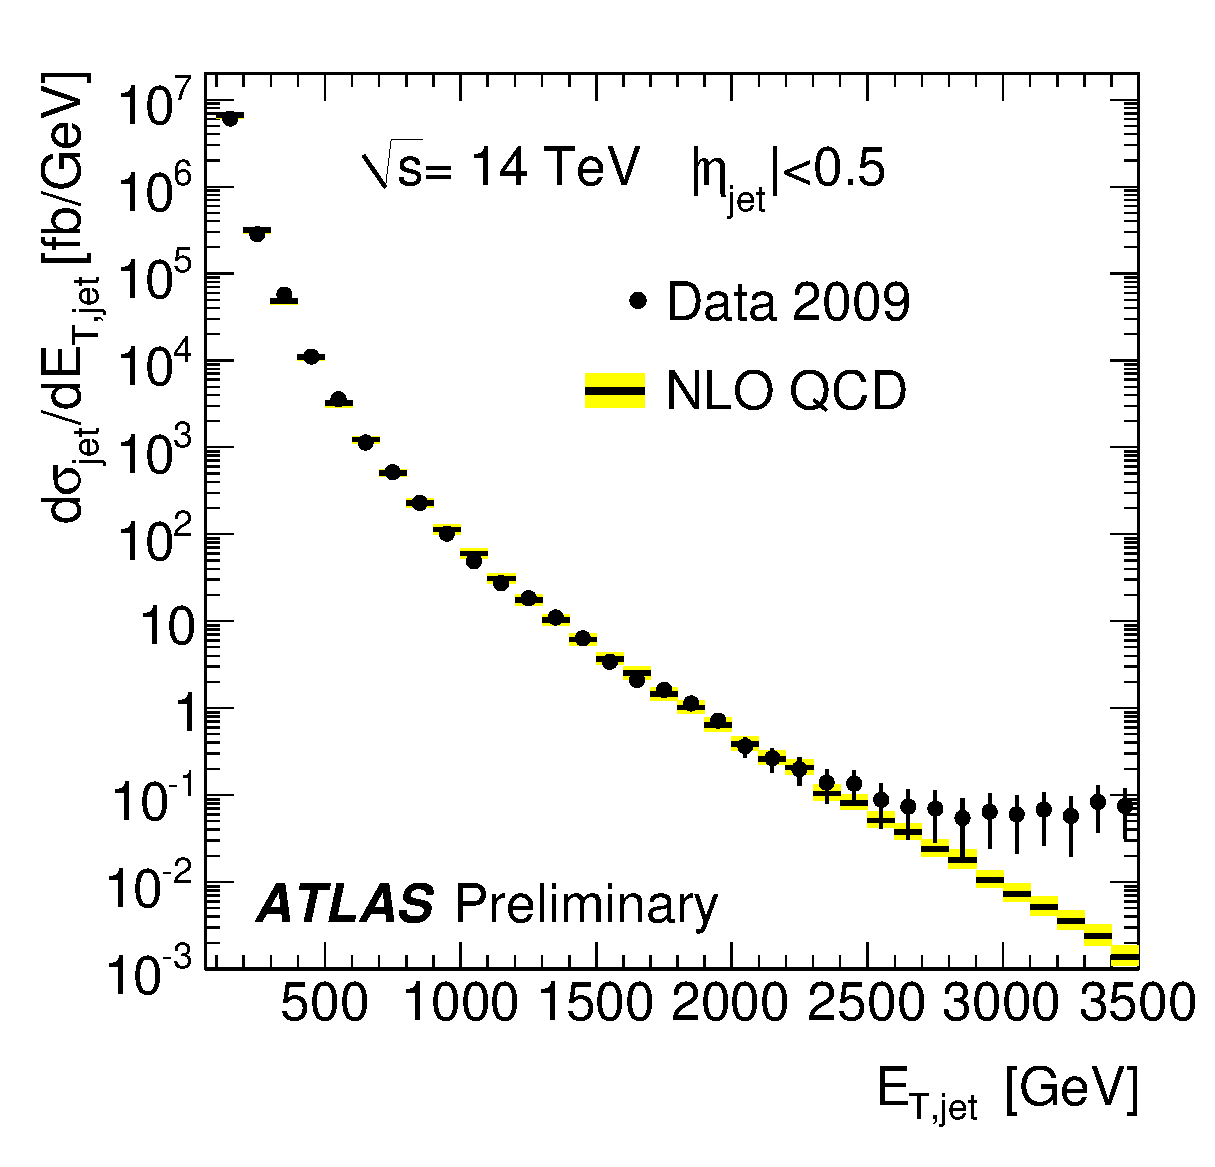
\includegraphics[width=0.5\columnwidth]{AtlasExample}
  \caption{An example ATLAS figure.}
  \label{fig:example}
\end{figure}

A figure with subfigures can be made as shown in the example of
Figure~\ref{fig:subfigexample}. In this example the \Package{subfig} package is used.
The syntax with the \Package{subcaption} and \Package{subfigure} packages is very similar.
The following commands were used to produce Figure~\ref{fig:subfigexample}:
{\footnotesize
\begin{verbatim}
\begin{figure}[htbp]
  \centering
  \subfloat[One subfigure example]{
    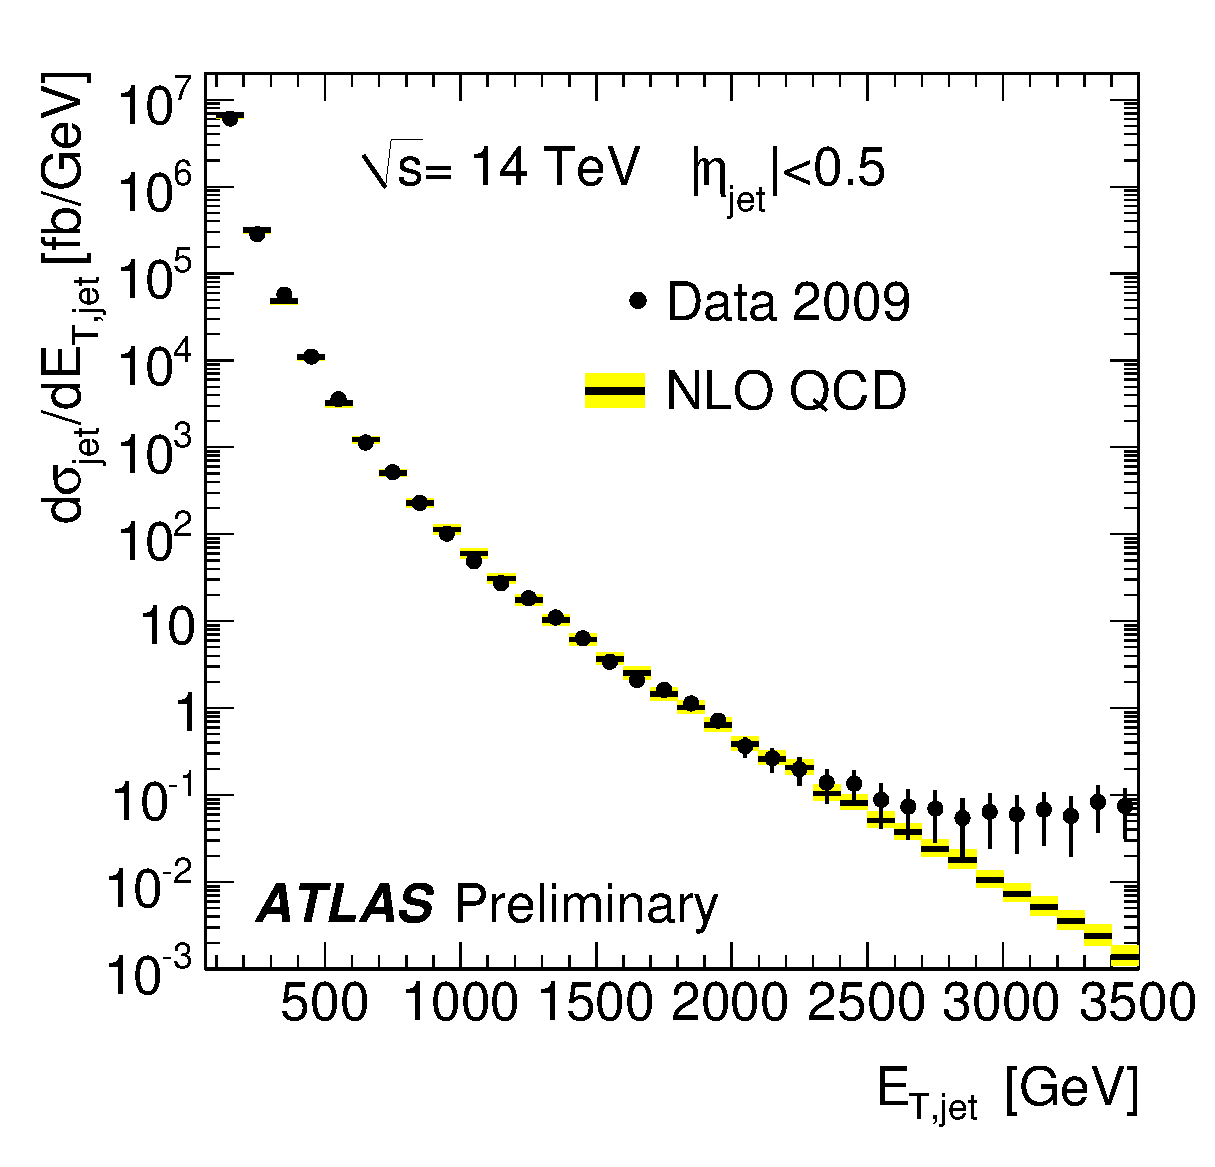
\includegraphics[width=0.45\textwidth]{AtlasExample}
    \label{fig:SubfigureExample1}
  }
  \subfloat[Another subfigure example]{
    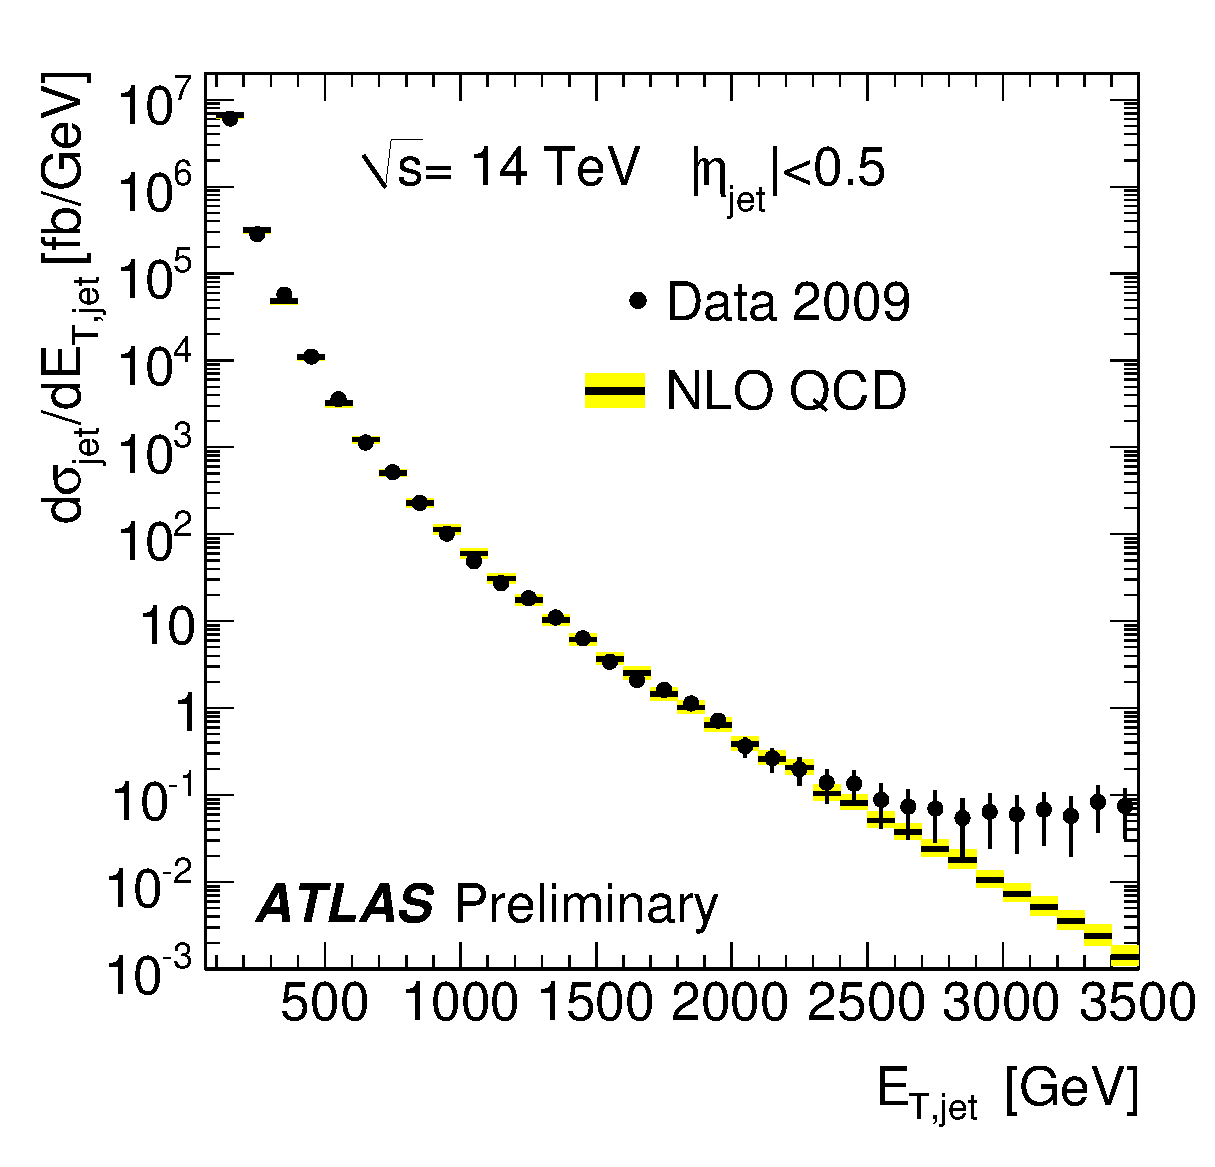
\includegraphics[width= 0.45\textwidth]{AtlasExample}
    \label{fig:SubfigureExample2}
  }
  \caption{Subfigure example.
    \protect\subref{fig:SubfigureExample1} shows the cross-section as a function of $E_{\text{T,jet}}$ and 
    \protect\subref{fig:SubfigureExample2} shows exactly the same thing!}
  \label{fig:subfigexample}
\end{figure}
\end{verbatim}
}

You refer to the main figure using the usual \verb|\ref| command, e.g.\ see \Fig{\ref{fig:subfigexample}}.
You can refer to the subfigures using either the syntax \verb|\ref{fig:subfiglabel}| 
(e.g.\ see \Fig{\ref{fig:SubfigureExample2}}) or\\
\verb|\ref{fig:mainfiglabel}\subref{fig:subfiglabel}|
(e.g.\ see \Fig{\ref{fig:subfigexample}\subref{fig:SubfigureExample1}}).
Note that if you use the \Package{subfig} package and want to use the labels of the subfigures in the caption,
you have to use the syntax \verb|\protect\subref{fig:SubfigureExample1}|.
The packages \Package{subfigure} and \Package{subcaption} do not need protect, but it does not do any harm.

\begin{figure}[htbp]
  \centering
  \subfloat[One subfigure example.]{
    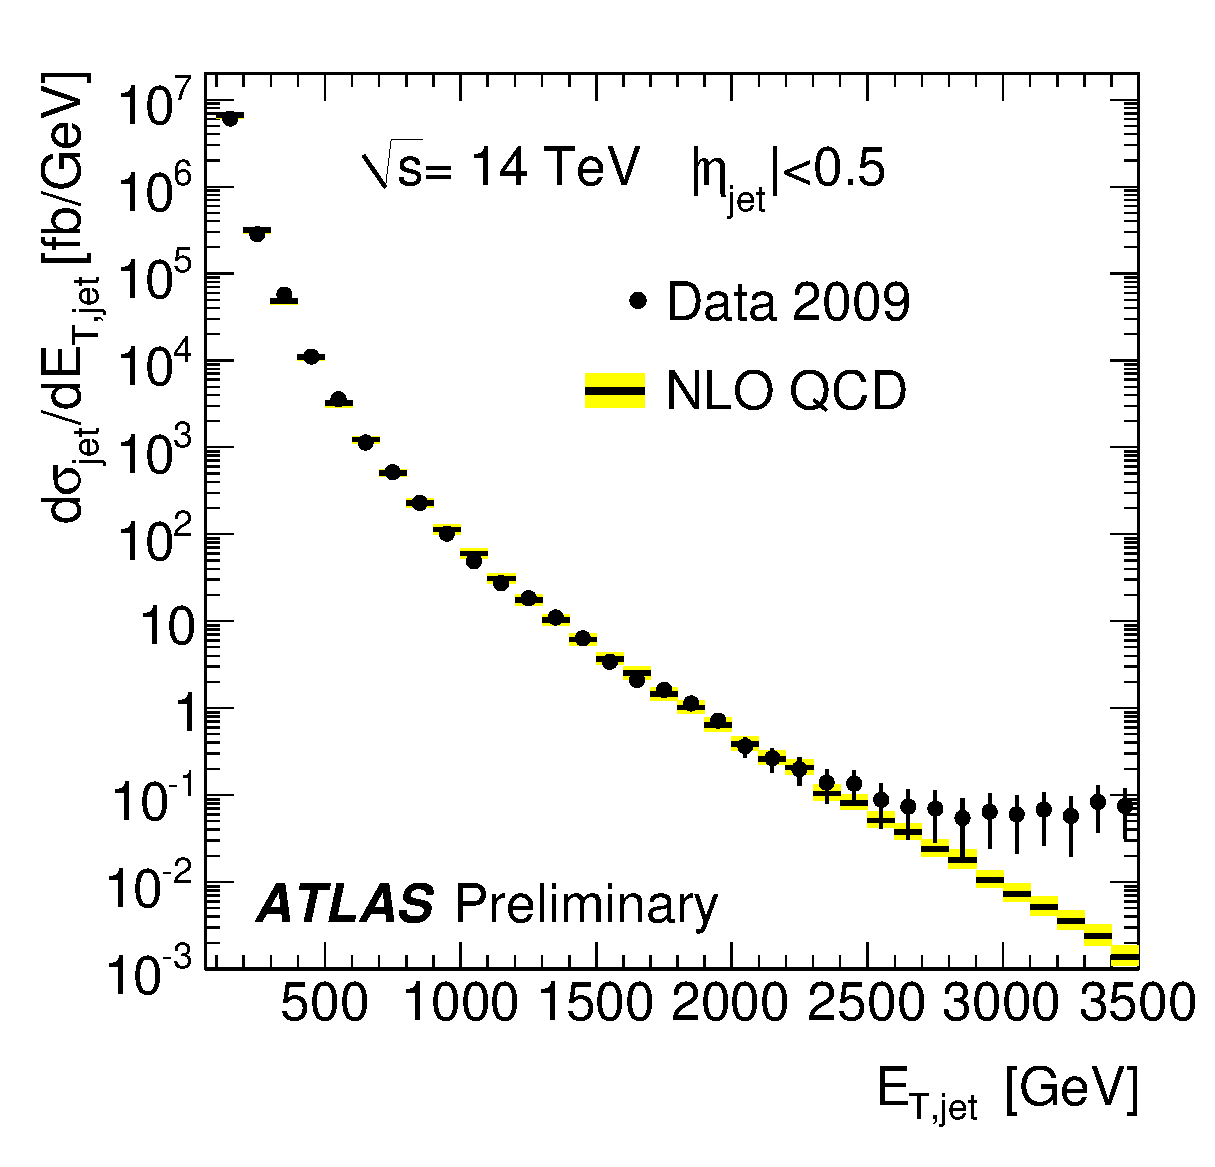
\includegraphics[width=0.45\textwidth]{AtlasExample}
    \label{fig:SubfigureExample1}
  }
  \subfloat[Another subfigure example.]{
    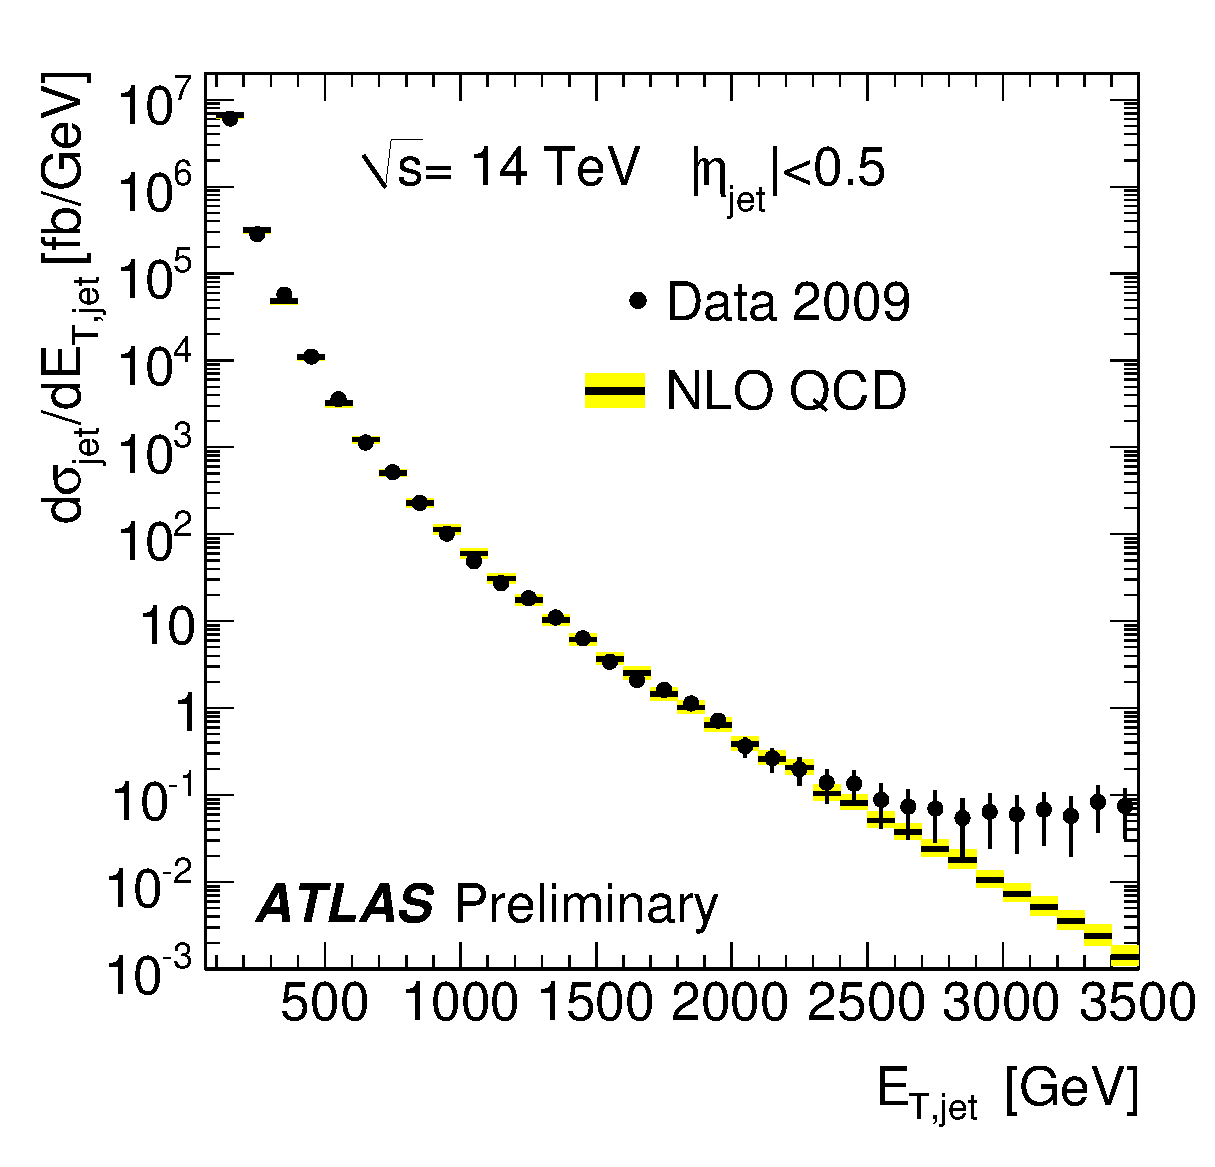
\includegraphics[width= 0.45\textwidth]{AtlasExample}
    \label{fig:SubfigureExample2}
  }
  \caption{Subfigure example.
    \protect\subref{fig:SubfigureExample1} shows the cross-section as a function of $E_{\text{T,jet}}$ and 
    \protect\subref{fig:SubfigureExample2} shows exactly the same thing!}
  \label{fig:subfigexample}
\end{figure}


%-------------------------------------------------------------------------------
\subsection{Positions of figures and tables}

In an ATLAS paper, all figures and tables should be printed before the conclusions.
You can achieve this by using the macro \Macro{FloatBarrier} from the
\Package{placeins} package.

In general, as mentioned above, you should separate the figure and table environments from the text by blank lines.
This helps the line numbers. The standard options to use for the placement are \Option{[htbp]}.


%-------------------------------------------------------------------------------
\subsection{\pT or \ET\ -- that is the question}

Bold math should be automatically invoked in titles.
This short section tests whether that works properly.
It is of course good if things like \pT and \ET are automatically in bold face in
a header and normal font in the text (and table of contents).

With the current setup, this works OK. 
However, if you just use the option \Option{koma}, which then typesets titles using a sans serif font,
the $p$ and $E$ are typeset with a serif font and \textsf{T} is typeset with a sans serif font,
which is probably not what one wants!
Work is still ongoing to find the optimal set of options
-- search for \texttt{detect} in the \Package{siunitx} manual, to see the complete set of possibilities.
This is not a problem for the ATLAS preprint style as it uses a serif font for the section titles.


%-------------------------------------------------------------------------------
\section{Remarks on units and symbols}

As discussed in the \enquote{General guidelines for ATLAS papers}~\cite{atlas-paper},
it is highly recommended to use a units package to format your units properly.
The package \Package{siunitx} works very well and is the package of choice.
Alternatives include \Package{units} and \Package{hepunits},
which is based on \Package{SIunits}.

The basic command to use in \Package{siunitx} is \verb|\SI{20}{\GeV}| to get
\SI{20}{\GeV}. 
There are also several other useful commands for specifying ranges:
\verb|\numrange| for a range of numbers and \verb|SIrange| for a range of numbers with a unit. 
Options exist for specifying how they are formatted.
The options can be set for an individual command or for the whole document.
For example, in this document I have specified the options:\\
\verb|\sisetup{separate-uncertainty, range-units=single, list=units=single}|
and\\
\verb|\sisetup{group-digits=integer, group-minimum-digits=4, detect-all}|.

In addition several extra units are defined:
\begin{itemize}
\item \verb|\micron| for \si{\micron};
\item \verb|\mrad| for \si{\mrad};
\item \verb|\nb| for \si{\nb};
\item \verb|\pb| for \si{\pb};
\item \verb|\fb| for \si{\fb}.
\end{itemize}
Use the syntax \verb|\SI{20.3}{\per\fb}| to get \SI{20.3}{\per\fb}.

Some things to note about using \Package{siunitx}:
\begin{itemize}
\item It tries to isolate itself from other packages.
  If you just want to write \si{\GeV} in your text,
  then you must write \verb|\si{\GeV}|.
\item It also contains two new column specifiers for tables ``S'' and ``s'',
  which are extremely useful for formatting tables properly.
\end{itemize}

The option names are somewhat different for \TeX\ Live 2009,
as this contained \Package{siunitx} Version 1.
You can use the older options by including \Package{atlaspackage} with the 
option \Option{texlive=2009}.
You also have to turn off the inclusion of \File{atlasunits.sty} by including the option \Option{units=false} with
the \Package{atlasphysics} package.


%-------------------------------------------------------------------------------
\section{From \texttt{atlasnote} to \texttt{atlasdoc}}
\label{sec:oldnote}
%-------------------------------------------------------------------------------

The \texttt{atlasdoc} class replaces and supersedes \texttt{atlasnote}.
The decision was taken to give the class a new name, as it is supposed to be
able to be used for (almost) all ATLAS documents.
Some small changes in the user setup are necessary to use the new
class, style files and templates.

All style files are collected in the \texttt{latex} subdirectory.
It is assumed that this directory is a direct subdirectory of you main \LaTeX\ file.
If you want to keep the style files in a central place you can either put them in
\verb|${HOME}/texmf/tex/latex| or create a link from your main directory to the location of
your \texttt{latex} directory.

The main changes the user has to make are:
\begin{itemize}
\item Change the class name from \texttt{atlasnote} to \texttt{latex/atlasdoc};
\item Specify the document language as an option: UKenglish or USenglish;
\item Add \verb|\usepackage{latex/atlaspackage}| at the beginning of the document;
\item Change \verb|\usepackage{atlasphysics}| to \verb|\usepackage{latex/atlasphysics}|; 
\item Use the macro \Macro{AtlasTitle} instead of \Macro{title}.
\end{itemize}

The language specification means that dates etc.\ are also formatted according to 
the document language. 
If you use the package \Macro{csquotes}, quotation symbols are also consistently and properly set
when you use \Macro{enquote}.

All the documentation now uses \texttt{biblatex} and \texttt{biber} instead of traditional \BibTeX.
The templates provide information on how to make the change in your own document.
The default document settings use \texttt{biblatex} and \texttt{bibtex}.

As of \File{atlaslatex-01-00-00} the same macro names are used in both \Package{atlasdoc} and
\Package{atlascover} so that title, journal, version number and abstract only need to be specified once.
This means that if you start from an old preamble the following changes should be made:
\begin{center}
  \begin{tabular}{ll}
    Old	& New\\
    \midrule
    \Macro{title} & \Macro{AtlasTitle}\\
    \Macro{draftversion} & \Macro{AtlasVersion}\\
    \Macro{atlasnote} & \Macro{AtlasNote}\\
    \Macro{journal} & \Macro{AtlasJournal}\\
    \Macro{abstracttext} & \Macro{AtlasAbstract}
  \end{tabular}
\end{center}
If you use the old macro names 
\Macro{draftversion}, \Macro{journal}, \Macro{abstracttext},
they will continue to work in the document itself, but not on the cover page.

When you want to circulate a draft with cover pages, 
you also need to set the macro \Macro{AtlasRefCode}.
This replaces \Macro{AtlasCoverNumber} as it is used in several places.

The class and style files have been cleaned up and things 
that were thought to no longer be necessary have been removed.
These pieces have been collected in \texttt{latex/atlasnote-obsolete.sty} in case they are needed.
If something important has got lost, please let me know.

The \Package{subfigure} package has been replaced with \Package{subfig}, as \Package{subfigure} is now deprecated.
If you use \Package{subfig}, then you have to use \Macro{subfloat} instead of \Macro{subfigure}.
If you want to continue to use \Package{subfigure} include \Package{atlaspackage} with the option
\Option{subfigure=true}. 
You should also comment out the \Macro{usepackage\{subfigure\}}.

Similarly, if you do not want to include \Package{siunitx} set
the option \Option{siunitx=false}.

The option \verb|\skipbeforetitle{<length>}| used to set the distance between
the title page header and the note title. 
Given that stretchable space is now used, such an option is no longer appropriate.
It can be given, but will be ignored.
%The default value should be fine for most notes, but in case you have a long list of
%authors or a lengthy abstract you can use this command to buy
%some extra space. Note that \verb|<length>| can also be negative
%(use it at your own risk!).


\appendix
%-------------------------------------------------------------------------------
\section{Journal templates}
%-------------------------------------------------------------------------------
\label{sec:journal}

This section contains some information on where the \LaTeX\ templates for the different journals can be found and how to use them.
However, with the advent of the ATLAS preprint style, 
it should no longer be necessary to format papers in the style used by the journals.
This section has therefore been moved to an appendix.

The directory \File{journal} contains a very basic paper outline with the preamble needed for different journals.
So far the \Package{atlaslatex} package has been tested with the classes for Elsevier and APS journals and the style file used for JHEP and JINST.
You should turn off the use of \Package{biblatex} if you use a journal template.
Add the option \Option{biblatex=false} to \Package{atlaspackage}.

\begin{description}
\item[Elsevier]Elsevier uses the \texttt{elsarticle} class which should be already installed if you have a standard 
  \TeX\ Live distribution. 
  It can also be found at \url{http://www.elsevier.com/locate/latex}.
  
\item[APS]APS journals use REV\TeX. This is also usually installed.
  It can also be found at \url{https://journals.aps.org/revtex}.
  Note that you have to specify the author after \verb|\begin{document}| with this class.
  Hence you should comment out the definition in your metadata file,\\
  e.g.\ \File{mydocument-metadata.tex}.
  If you want line numbers in a document typeset using REV\TeX, it is best to use the class option \Option{linenumbers}.
  In addition you should include \Package{atlaspackage} with the option \Option{lineno=false}.
  
\item[JHEP]The package can be downloaded from \url{http://jhep.sissa.it/jhep/help/JHEP_TeXclass.jsp}. It contains a style file \File{jheppub.sty} as well as a \BibTeX\ style file \File{JHEP.bst}. 
\end{description}


%-------------------------------------------------------------------------------
\section{History}
%-------------------------------------------------------------------------------

Quite a lot of people have contributed to the ATLAS \LaTeX\ templates over time.
Marco Delmastro set them up in the first place and added a number of improvements over time.
Mike Vetterli implemented several changes to the cover pages, including switching to two pages.
Cristina Oropeza, Vasia Mitsou, Chris Hays and Mike Vetterli all made contributions to the preprint cover page.

Sven Menke provided the code so that bold math works in titles correctly.
Thorsten Kuhl had the idea of defining \Macro{ATLASLATEXPATH}, which makes things much more flexible.

%-------------------------------------------------------------------------------
\subsection{Changes in \texttt{atlaslatex-02-00-00}}
\label{sec:atlaslatex2}
%-------------------------------------------------------------------------------

As of Version 02-00-00 of \Package{atlaslatex}, only the \KOMAScript\ classes are supported.
At the same time, the option BOOK was introduced, which uses \Package{scrbook} as the base class.
This is more suitable for long documents such as a TDR.

Several options, which make maintenance more difficult have been removed:
\Option{maketitle}, \Option{nomaketitle}, \Option{koma}.
In addition, support for \TeX\ Live versions older than 2009 has been removed.
A version of the class with these options, which should still work with \TeX\ Live 2007,
but without the \Option{BOOK} option is available as \File{atlasdoc1.cls}.
However, the class (\Package{atlasdoc1}) will not be actively maintained or developed any more.
If you want to explicitly load the \Package{atlascover} package,
you should load \Package{atlascover1} when using \Package{atlasdoc1}.

The options \Option{cernpreprint}, \Option{preprint} and \Option{auxmat} are no longer available
in \Package{atlascover}.
You should pass these to \Package{atlasdoc} instead, as the title pages are now part of the main class.


%-------------------------------------------------------------------------------
\subsection{Changes in \texttt{atlascover-01-00-00}}
\label{sec:oldcover}
%-------------------------------------------------------------------------------

As of \Package{atlascover-01-00-00} the same macro names are used in both \Package{atlasdoc} and
\Package{atlascover} so that title, journal and version number only need to be specified once.
This means that if you start from an old cover page the following changes have to be made:
\begin{center}
  \begin{tabular}{ll}
    Old                            & New                   \\
    \midrule
    \Macro{AtlasCoverPaperTitle}   & \Macro{AtlasTitle}    \\
    \Macro{AtlasCoverNumber}       & \Macro{AtlasRefCode}  \\
    \Macro{AtlasCoverPaperVersion} & \Macro{AtlasVersion}  \\
    \Macro{AtlasCoverJournal}      & \Macro{AtlasJournal}  \\
    \Macro{AtlasCoverAbstract}     & \Macro{AtlasAbstract}
  \end{tabular}
\end{center}

Note that \Package{atlaspreprint} is integrated into \Package{atlascover} and not maintained as a separate style file.
To get the CERN preprint front page, you have to include the option \Option{cernpreprint} when you invoke \Package{atlasdoc}.
If you start from an old preprint front page the following changes have to be made:
\begin{center}
  \begin{tabular}{ll}
    Old                              & New                   \\
    \midrule
    \Macro{PreprintCoverPaperTitle} & \Macro{AtlasTitle}    \\
    \Macro{PreprintJournalName}     & \Macro{AtlasJournal}  \\
    \Macro{PreprintCoverAbstract}   & \Macro{AtlasAbstract}
  \end{tabular}
\end{center}
The following changes are needed for the macros:
\begin{itemize}
\item The macro \Macro{AtlasCoverEdBoardMember} only has one argument, as a generic email list now exists for every EdBoard.
\end{itemize}


